\scanpage{108}

\figure{%
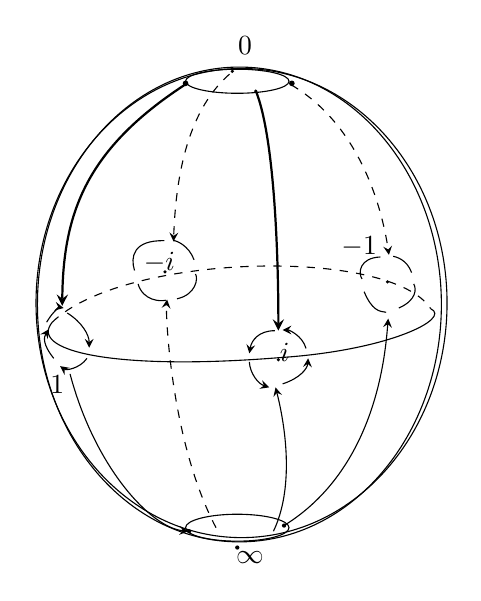
\begin{tikzpicture}[x=0.9cm,y=0.9cm,>=stealth]
\draw[thin] (0,0) ellipse (2.85 and 3.35);
\draw[thin] (0.03,0.02) ellipse (2.9 and 3.31);
\draw (-0.03,3.15) ellipse (0.73 and 0.17);
\draw (-0.03,-3.15) ellipse (0.73 and 0.19);
\node at (0.08,3.65) {$0$};
\node at (0.15,-3.57) {$\infty$};
\draw[dashed] (-2.64,-0.25) .. controls (-1.65,0.72) and (2.13,0.82) .. (2.7,-0.06);
\draw (-2.64,-0.25) .. controls (-2.98,-0.65) and (-1.8,-0.94) .. (0.57,-0.75) .. controls (2.1,-0.65) and (3.0,-0.2) .. (2.7,-0.06);
\draw[->,thick] (-0.77,3.1) .. controls (-2.15,2.2) and (-2.49,1.3) .. (-2.5,-0.02);
\draw[->] (-2.39,-0.98) .. controls (-2.04,-2.3) and (-1.25,-3.15) .. (-0.72,-3.2);
\draw[->,thick] (0.23,3.02) .. controls (0.5,2.35) and (0.55,0.65) .. (0.55,-0.37);
\draw[->] (0.48,-3.2) .. controls (0.76,-2.62) and (0.67,-1.8) .. (0.51,-1.17);
\draw[dashed,->] (-0.14,3.25) .. controls (-0.77,2.7) and (-0.9,1.7) .. (-0.93,0.89);
\draw[dashed,->] (-0.33,-3.15) .. controls (-0.98,-1.91) and (-1.04,-0.1) .. (-1.02,0.07);
\draw[dashed,->] (0.73,3.1) .. controls (1.75,2.5) and (2.03,1.25) .. (2.11,0.7);
\draw[->] (0.63,-3.12) .. controls (1.94,-2.31) and (2.06,-0.68) .. (2.1,-0.2);
\draw[->] (-2.43,-0.12) .. controls (-2.22,-0.25) and (-2.12,-0.43) .. (-2.12,-0.61);
\draw[->] (-2.15,-0.76) .. controls (-2.26,-0.91) and (-2.45,-0.93) .. (-2.53,-0.87);
\draw[->] (-2.62,-0.76) .. controls (-2.78,-0.56) and (-2.76,-0.46) .. (-2.69,-0.35);
\draw[->] (-2.72,-0.25) .. controls (-2.62,-0.08) and (-2.53,-0.04) .. (-2.48,-0.05);
\node at (-2.57,-1.13) {$1$};
\draw[->] (0.5,-0.37) .. controls (0.27,-0.37) and (0.17,-0.51) .. (0.14,-0.69);
\draw[->] (0.14,-0.81) .. controls (0.15,-0.98) and (0.27,-1.12) .. (0.42,-1.17);
\draw[->] (0.61,-1.12) .. controls (0.86,-1.04) and (0.96,-0.9) .. (0.97,-0.76);
\draw[->] (0.94,-0.62) .. controls (0.89,-0.44) and (0.7,-0.36) .. (0.61,-0.36);
\node at (0.64,-0.68) {$i$};
\fill (0.55,-0.78) circle (0.025);
\draw (-1.06,0.9) .. controls (-1.5,0.91) and (-1.54,0.67) .. (-1.48,0.48);
\draw (-1.43,0.29) .. controls (-1.36,0.05) and (-1.11,0.04) .. (-1.04,0.06);
\draw (-0.88,0.08) .. controls (-0.61,0.14) and (-0.58,0.37) .. (-0.62,0.43);
\draw (-0.64,0.63) .. controls (-0.71,0.83) and (-0.9,0.91) .. (-0.93,0.9);
\node at (-1.13,0.59) {$-i$};
\fill (-1.05,0.46) circle (0.025);
\draw (1.99,0.67) .. controls (1.7,0.66) and (1.67,0.45) .. (1.73,0.36);
\draw (1.76,0.18) .. controls (1.87,-0.08) and (1.97,-0.1) .. (2.07,-0.11);
\draw (2.25,-0.05) .. controls (2.5,0.06) and (2.5,0.22) .. (2.46,0.29);
\draw (2.43,0.45) .. controls (2.36,0.64) and (2.21,0.67) .. (2.17,0.68);
\node at (1.69,0.81) {$-1$};
\fill (2.09,0.32) circle (0.025);
\fill (-0.76,3.12) circle (0.04);\fill (0.74,3.12) circle (0.04);
\fill (-0.1,3.29) circle (0.025);\fill (0.23,3.01) circle (0.025);
\fill (-0.71,-3.2) circle (0.03);\fill (0.63,-3.12) circle (0.03);
\fill (-0.03,-3.43) circle (0.03);
\end{tikzpicture}%
}

\diagram{\begin{tikzcd}[ampersand replacement=\&,row sep=small]
z \arrow[r] \& -z \\
z \arrow[r] \& \dfrac{1}{z} \\
\unsure{z} \& {} \arrow[l]
\end{tikzcd}}

\diagram{\begin{tikzcd}[ampersand replacement=\&]
1 \arrow[r] \& \mathbb{F}_2^2 \arrow[r] \& A_4 \arrow[r] \& \mathbb{Z}/3\mathbb{Z} \arrow[r] \& 1
\end{tikzcd}}

\figure{%
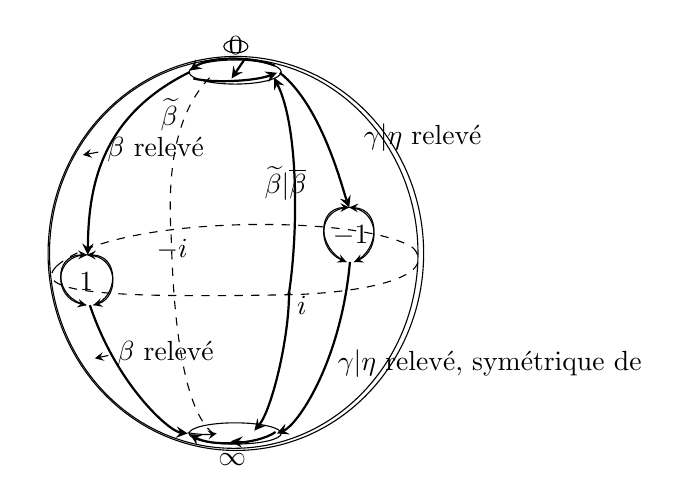
\begin{tikzpicture}[x=0.9cm,y=0.9cm,>=stealth]
\draw[thin] (0,0) ellipse (2.6 and 2.75);
\draw[thin] (0.03,0) ellipse (2.65 and 2.78);
\draw (0.02,2.56) ellipse (0.65 and 0.17);
\draw (0.02,-2.54) ellipse (0.65 and 0.15);
\node at (0.03,2.93) {$\unsure{0}$};
\draw (0.03,2.92) ellipse (0.17 and 0.09);
\node at (-0.02,-2.91) {$\infty$};
\draw[dashed] (-2.5,-0.18) .. controls (-1.7,0.55) and (1.8,0.56) .. (2.53,0.08);
\draw[dashed] (-2.5,-0.18) .. controls (-2.9,-0.58) and (-1.6,-0.63) .. (0.9,-0.58) .. controls (2.2,-0.52) and (2.84,-0.25) .. (2.53,0.08);
\draw[->,thick] (-0.62,2.56) .. controls (-1.9,1.93) and (-2.05,0.91) .. (-2.06,-0.02);
\draw[->,thick] (-2.03,-0.73) .. controls (-1.65,-1.86) and (-0.91,-2.51) .. (-0.65,-2.54);
\draw[->,thick] (0.65,2.55) .. controls (1.25,2.08) and (1.54,0.89) .. (1.63,0.65);
\draw[->,thick] (1.64,-0.12) .. controls (1.51,-1.54) and (0.9,-2.42) .. (0.61,-2.54);
\draw[dashed] (-0.34,2.48) .. controls (-0.93,1.87) and (-0.92,0.84) .. (-0.88,0.18) .. controls (-0.84,-1.3) and (-0.64,-2.26) .. (-0.3,-2.53);
\draw[->] (-0.65,-2.53) .. controls (-0.4,-2.57) and (-0.3,-2.55) .. (-0.24,-2.54);
\draw[->,thick] (0.78,-0.56) .. controls (0.91,0.3) and (0.92,1.78) .. (0.57,2.48);
\draw[->,thick] (0.78,-0.56) .. controls (0.78,-1.22) and (0.53,-2.22) .. (0.29,-2.5);
\draw[->] (-2.07,-0.02) .. controls (-2.55,-0.02) and (-2.55,-0.62) .. (-2.08,-0.73);
\draw[->] (-2.07,-0.02) .. controls (-1.61,-0.03) and (-1.62,-0.62) .. (-1.98,-0.73);
\draw[->] (-2.08,-0.73) .. controls (-2.55,-0.62) and (-2.55,-0.02) .. (-2.07,-0.02);
\draw[->] (-1.98,-0.73) .. controls (-1.62,-0.62) and (-1.61,-0.03) .. (-2.07,-0.02);
\node at (-2.08,-0.39) {$1$};
\draw[->] (1.63,0.65) .. controls (1.17,0.64) and (1.17,0.06) .. (1.59,-0.12);
\draw[->] (1.63,0.65) .. controls (2.08,0.62) and (2.06,0.04) .. (1.7,-0.12);
\draw[->] (1.59,-0.12) .. controls (1.17,0.06) and (1.17,0.64) .. (1.63,0.65);
\draw[->] (1.7,-0.12) .. controls (2.06,0.04) and (2.08,0.62) .. (1.63,0.65);
\node at (1.65,0.25) {$-1$};
\node at (-0.87,0.05) {$-i$};
\fill (0.78,-0.56) circle (0.025);\node at (0.96,-0.73) {$i$};
\node at (-0.91,1.96) {$\widetilde{\beta}$};
\node at (0.73,0.99) {$\unsure{\widetilde{\beta}|\overline{\beta}}$};
\node[anchor=west] at (-1.92,1.46) {$\beta$ relevé};
\draw[->] (-1.91,1.43) -- (-2.13,1.39);
\node[anchor=west] at (-1.78,-1.41) {$\beta$ relevé};
\draw[->] (-1.77,-1.44) -- (-1.96,-1.48);
\node[anchor=west] at (1.7,1.64) {$\unsure{\gamma|\eta}$ relevé};
\node[anchor=west] at (1.33,-1.55) {$\unsure{\gamma|\eta}$ relevé, \unsure{symétrique de}};
\draw[->,thick] (0.58,2.65) .. controls (0.2,2.8) and (-0.36,2.77) .. (-0.62,2.58);
\draw[->,thick] (-0.57,2.47) .. controls (-0.3,2.4) and (0.3,2.43) .. (0.61,2.55);
\draw[->,thick] (0.14,2.72) -- (-0.03,2.47);
\draw[->,thick] (0.59,-2.52) .. controls (0.31,-2.71) and (-0.33,-2.72) .. (-0.62,-2.55);
\draw[->,thick] (0.21,-2.67) -- (-0.04,-2.65);
\end{tikzpicture}%
}

\[
l_{\infty}l_1l_0l_{-1}=1
\]

\mspage{107}
